%%%%%%%%%%%%%%%%%%%%%%%%%%%%%%%%%%%%%%%%%%%%%%%%%%%%%%%%%%%%%%%%%%%%
%% %%	Posterdown PDF class for LaTeX files	 08-JAN-2019
%% %%	For any information please send an e-mail to:
%% %%		brentthonre18@gmail.com (Brent Thorne)
%% %%
%% %%	Initial class provided by:
%% %%		Brent Thorne
%% %% Contributors: Shea Connell (SC)
%%%%%%%%%%%%%%%%%%%%%%%%%%%%%%%%%%%%%%%%%%%%%%%%%%%%%%%%%%%%%%%%%%%%

\documentclass[article,30pt,extrafontsizes]{memoir}

%utf-8 seems to be important
\RequirePackage[utf8]{inputenc}
\RequirePackage[T1]{fontenc}
\RequirePackage{lmodern}
\RequirePackage{multicol}
\RequirePackage{graphicx}
\RequirePackage{lipsum}
\RequirePackage{blindtext}
\RequirePackage[svgnames,table]{xcolor}
\RequirePackage{tikz}
\RequirePackage[framemethod=tikz]{mdframed}
\RequirePackage{color}
\RequirePackage{geometry}
\RequirePackage{adjmulticol}
\RequirePackage[skins,most,listings,skins]{tcolorbox}

%For kable extra package :)
\RequirePackage{booktabs}
\RequirePackage{longtable}
\RequirePackage{array}
\RequirePackage{multirow}
\RequirePackage{wrapfig}
\RequirePackage{float}
\RequirePackage{colortbl}
\RequirePackage{pdflscape}
\RequirePackage{pagecolor}
\RequirePackage{tabu}
\RequirePackage{threeparttable}
\RequirePackage{threeparttablex}
\RequirePackage[normalem]{ulem}
\RequirePackage{makecell}
\RequirePackage{wrapfig}

%rof hyperrefs
\RequirePackage{hyperref}
\hypersetup{
    colorlinks=true,
    linkcolor=linkcol,
    citecolor=citecol,
    filecolor=linkcol,
    urlcolor=urlcol,
}
%For figure and table placement
\RequirePackage{float}
\floatplacement{figure}{H}
\floatplacement{table}{H}

%%%%%%%%% COLOURS %%%%%%%%
%Fill/ Line Colours
\definecolor{titleboxbgcol}{HTML}{008080}
\definecolor{titleboxbordercol}{HTML}{0b4545}
\definecolor{columnlinecol}{HTML}{008080}
\definecolor{bodybgcol}{HTML}{ffffff}
\definecolor{sectitlebgcol}{HTML}{0b4545}
\definecolor{sectitlebordercol}{HTML}{0b4545}
% Text Colours
\definecolor{titletextcol}{HTML}{ffffff}
\definecolor{authortextcol}{HTML}{0b4545}
\definecolor{affiliationtextcol}{HTML}{FFFFFF}
\definecolor{sectitletextcol}{HTML}{ffffff}
\definecolor{bodytextcol}{HTML}{000000}
\definecolor{footnotetextcol}{HTML}{ffffff}
\definecolor{citecol}{HTML}{CC0000}
\definecolor{urlcol}{HTML}{008080}
\definecolor{linkcol}{HTML}{008080}


%Memoir spacing options
%spacing between figure/ table and caption
\setlength{\abovecaptionskip}{0.4in}
\setlength{\belowcaptionskip}{0.2in}
\captionnamefont{\footnotesize\sffamily\bfseries}
\captiontitlefont{\footnotesize\sffamily}

%define column options
\setlength{\columnseprule}{0pt}
\def\columnseprulecolor{\color{columnlinecol}}

%define section title features
\setsubsubsecheadstyle{\small\color{sectitletextcol}\textbf}% Set \section style
\setsecnumformat{}
\def\sectionmark#1{\markboth{#1}{#1}}

%%%%%%%%%%%% TCOLORBOXES TO THE RESCUE %%%%%%%%%%%%%%%%%%%%
%Title Box
\newtcolorbox{topbox}{
enhanced,
colback=titleboxbgcol,
colframe=titleboxbordercol,
halign=center,
boxrule=1cm,
sharp corners=all,
 overlay={
    \node[anchor=south west]
      at ([xshift=1in,yshift=1in]frame.south west)
       {
\includegraphics[width=3in]{Figures/batpig}};
    \node[anchor=south east]
      at ([xshift=-1in,yshift=1in]frame.south east)
       {
\includegraphics[width=3in]{Figures/batpig}};}

}
%Body Section Title Box
\newtcolorbox{myboxstuff}[1][]{
code={\parindent=0em},
colframe=sectitlebordercol,
nobeforeafter,
left skip=0pt,
valign=center,
halign=center,
fontupper=\Large\bfseries,
colupper=sectitletextcol,
boxrule=2mm,
colback=sectitlebgcol,
sharp corners=uphill, #1}
\newcommand{\mybox}[1]{%
\begin{myboxstuff}
\strut #1
\end{myboxstuff}%
}
\makeheadstyles{MyBox}{
    \setsecheadstyle{\mybox}
}
\headstyles{MyBox}\makepagestyle{MyBox}
%-----------------------------------------------------
%Make sure that the page is empty of any preset items from memoir
\thispagestyle{empty}

%biblatex options
\RequirePackage[sorting=none,backend=biber]{biblatex}
\renewcommand*{\bibfont}{\small} %% SC
\bibliography{biblio}
\defbibheading{bibliography}[\bibname]{%
\setlength\bibitemsep{0.8\itemsep} %% SC
\section*{#1}%
\markboth{#1}{#1}}
\AtBeginDocument{%
  \renewcommand{\bibname}{References}
}

%Remove section numbering & set 2nd level header as first level
%to avoid the automatic new page generated from memoir chapter
%formatting
\counterwithout{section}{chapter}
\makechapterstyle{mydefault}{
\addtocounter{secnumdepth}{2}
\setsecheadstyle{\mybox}
\setsubsecheadstyle{\itshape}
\setsubsubsecheadstyle{\itshape}
}

%set the chapterstyle
\chapterstyle{mydefault}

%define column spacing
\setlength\columnsep{0.5in}

%spacing params
\setlength\parindent{0em}
\setlength\parskip{0em}
\setlength\hangparas{0}

%spacing after section head title
\setaftersecskip{0em}
\setbeforesecskip{1.5em}
\setlength\textfloatsep{0in}
\setlength\floatsep{0in}
\setlength\intextsep{0in}

\setstocksize{38in}{45in}
\settrimmedsize{\stockheight}{\stockwidth}{*}
\settypeblocksize{38in}{45in}{*}
\setlrmargins{*}{*}{1}
\setulmarginsandblock{2.5cm}{*}{*}
\setmarginnotes{0em}{0cm}{0cm}
\setlength{\footskip}{0cm}
\setlength{\footnotesep}{0cm}
\setlength{\headheight}{0pt}
\setlength{\headsep}{0pt}
\setlength{\trimtop}{0pt}
\setlength{\trimedge}{0pt}
\setlength{\uppermargin}{0pt}
\checkandfixthelayout

%Footnote to white
\RequirePackage{footmisc}
\def\footnotelayout{\centering\color{footnotetextcol}}

% see https://stackoverflow.com/a/47122900
\usepackage{color}
\usepackage{fancyvrb}
\newcommand{\VerbBar}{|}
\newcommand{\VERB}{\Verb[commandchars=\\\{\}]}
\DefineVerbatimEnvironment{Highlighting}{Verbatim}{commandchars=\\\{\}}
% Add ',fontsize=\small' for more characters per line
\usepackage{framed}
\definecolor{shadecolor}{RGB}{248,248,248}
\newenvironment{Shaded}{\begin{snugshade}}{\end{snugshade}}
\newcommand{\AlertTok}[1]{\textcolor[rgb]{0.94,0.16,0.16}{#1}}
\newcommand{\AnnotationTok}[1]{\textcolor[rgb]{0.56,0.35,0.01}{\textbf{\textit{#1}}}}
\newcommand{\AttributeTok}[1]{\textcolor[rgb]{0.77,0.63,0.00}{#1}}
\newcommand{\BaseNTok}[1]{\textcolor[rgb]{0.00,0.00,0.81}{#1}}
\newcommand{\BuiltInTok}[1]{#1}
\newcommand{\CharTok}[1]{\textcolor[rgb]{0.31,0.60,0.02}{#1}}
\newcommand{\CommentTok}[1]{\textcolor[rgb]{0.56,0.35,0.01}{\textit{#1}}}
\newcommand{\CommentVarTok}[1]{\textcolor[rgb]{0.56,0.35,0.01}{\textbf{\textit{#1}}}}
\newcommand{\ConstantTok}[1]{\textcolor[rgb]{0.00,0.00,0.00}{#1}}
\newcommand{\ControlFlowTok}[1]{\textcolor[rgb]{0.13,0.29,0.53}{\textbf{#1}}}
\newcommand{\DataTypeTok}[1]{\textcolor[rgb]{0.13,0.29,0.53}{#1}}
\newcommand{\DecValTok}[1]{\textcolor[rgb]{0.00,0.00,0.81}{#1}}
\newcommand{\DocumentationTok}[1]{\textcolor[rgb]{0.56,0.35,0.01}{\textbf{\textit{#1}}}}
\newcommand{\ErrorTok}[1]{\textcolor[rgb]{0.64,0.00,0.00}{\textbf{#1}}}
\newcommand{\ExtensionTok}[1]{#1}
\newcommand{\FloatTok}[1]{\textcolor[rgb]{0.00,0.00,0.81}{#1}}
\newcommand{\FunctionTok}[1]{\textcolor[rgb]{0.00,0.00,0.00}{#1}}
\newcommand{\ImportTok}[1]{#1}
\newcommand{\InformationTok}[1]{\textcolor[rgb]{0.56,0.35,0.01}{\textbf{\textit{#1}}}}
\newcommand{\KeywordTok}[1]{\textcolor[rgb]{0.13,0.29,0.53}{\textbf{#1}}}
\newcommand{\NormalTok}[1]{#1}
\newcommand{\OperatorTok}[1]{\textcolor[rgb]{0.81,0.36,0.00}{\textbf{#1}}}
\newcommand{\OtherTok}[1]{\textcolor[rgb]{0.56,0.35,0.01}{#1}}
\newcommand{\PreprocessorTok}[1]{\textcolor[rgb]{0.56,0.35,0.01}{\textit{#1}}}
\newcommand{\RegionMarkerTok}[1]{#1}
\newcommand{\SpecialCharTok}[1]{\textcolor[rgb]{0.00,0.00,0.00}{#1}}
\newcommand{\SpecialStringTok}[1]{\textcolor[rgb]{0.31,0.60,0.02}{#1}}
\newcommand{\StringTok}[1]{\textcolor[rgb]{0.31,0.60,0.02}{#1}}
\newcommand{\VariableTok}[1]{\textcolor[rgb]{0.00,0.00,0.00}{#1}}
\newcommand{\VerbatimStringTok}[1]{\textcolor[rgb]{0.31,0.60,0.02}{#1}}
\newcommand{\WarningTok}[1]{\textcolor[rgb]{0.56,0.35,0.01}{\textbf{\textit{#1}}}}

% choose font family
\RequirePackage{palatino}

% define the BODYBGCOL
\newpagecolor{bodybgcol}

%sets footnote to be white hopefully
\renewcommand\footnoterule{}
\renewcommand{\thempfootnote}{\footnotesize\color{footnotetextcol}{\arabic{mpfootnote}}}

%-------------- Begin Document -------------------%
\begin{document}

%-------------- Title Box Start ------------------%
%tcolorbox allows for pictures hopefully
\begin{topbox}
  \color{titletextcol}
  \vspace{0.5in}
  \Huge{\fontfamily{phv}\selectfont escaping batpigday}  \\[0.3in]  %% SC
  \color{authortextcol} \Large{Charles T. Gray\textsuperscript{1}} \\[0.2in] %% SC
  \color{affiliationtextcol} \large{\textsuperscript{1}Department of Mathematics and Statistics, La Trobe
University, Victoria, Australia} %% SC
  \vspace{1cm}
\end{topbox}
%--------------- Title Box End -------------------%
%----------------- Body Start --------------------%
% Begin body of poster
\begin{adjmulticols*}{3}{0.5in}{0.5in}
\normalsize{  %% SC
\color{bodytextcol}
\hypertarget{batpigday}{%
\section{batpigday}\label{batpigday}}

\begin{description}
  \item[batpigday]{\emph{noun} The coding equivalent of groundhogday.}
\end{description}

\hypertarget{the-problem}{%
\section{the problem}\label{the-problem}}

\begin{center}\rule{0.5\linewidth}{\linethickness}\end{center}

\begin{center}
Simulating data is a bitch. 
\end{center}

\begin{center}\rule{0.5\linewidth}{\linethickness}\end{center}

Debugging frequently dominates the time of students in mathematical
science. These students know how to solve equations, and next to nothing
about code.

\begin{center}\rule{0.5\linewidth}{\linethickness}\end{center}

New tools\autocite{wickham_tidyverse:_2017} are emerging daily to enable
researchers to avoid these timesink pitfalls.

These tools have lowered the programmatic barrier for researchers, but
it still a learning curve.

\begin{center}\rule{0.5\linewidth}{\linethickness}\end{center}

We consider a case study in meta-analysis.

\begin{description}
\item[meta-analysis] Statistical methodology for combining the results of several studies. 

\end{description}

\hypertarget{meta-analysis-of-medians}{%
\section{meta-analysis of medians}\label{meta-analysis-of-medians}}

Conventional meta-analytic tools, such as
\texttt{metafor::rma}\autocite{viechtbauer_conducting_2010}, require an
\textbf{effect} and a \textbf{variance} of that effect.

\begin{center}\rule{0.5\linewidth}{\linethickness}\end{center}

But what if the reported statistics are \textbf{median} and
\textbf{interquartile} range? Existing estimators, such as
\autocite{wan_estimating_2014}, estimate a mean and standard deviation.

\begin{center}\rule{0.5\linewidth}{\linethickness}\end{center}

To test our proposed estimator for the variance of the sample median, I
found myself repeating tasks and checks in the algorithms.

\begin{center}\rule{0.5\linewidth}{\linethickness}\end{center}

I tried to find a better way of debugging and writing simulations.

This lead to:

\begin{enumerate}
\def\labelenumi{\arabic{enumi}.}
\tightlist
\item
  a packaged analysis\autocite{marwick_packaging_2018},
  \texttt{varameta::}*, which is built on
\item
  the simulation package for meta-analysis data, \texttt{metasim::}*.
\end{enumerate}

(*in development)

\begin{center}
\textbf{coding is the easiest part of coding}
\end{center}

\begin{itemize}
\tightlist
\item
  Modular code with functions rather than script
\item
  Reproducibility is more than \texttt{set.seed()}
\item
  Versioning and collaboration via Git
\item
  Packaged analyses
\end{itemize}

\columnbreak

\hypertarget{escaping-batpigday}{%
\section{escaping batpigday}\label{escaping-batpigday}}

Generate sample sizes for \(k\) studies.

\begin{Shaded}
\begin{Highlighting}[]
\KeywordTok{library}\NormalTok{(tidyverse)}
\KeywordTok{library}\NormalTok{(metasim)}
\end{Highlighting}
\end{Shaded}

\begin{Shaded}
\begin{Highlighting}[]
\CommentTok{# simulate 2 studies where most have at most 25}
\KeywordTok{sim_n}\NormalTok{(}\DataTypeTok{k =} \DecValTok{2}\NormalTok{, }\DataTypeTok{min_n =} \DecValTok{10}\NormalTok{, }\DataTypeTok{max_n =} \DecValTok{25}\NormalTok{) }\OperatorTok\StringTok{ }\KeywordTok{output_table}\NormalTok{()}
\end{Highlighting}
\end{Shaded}

\rowcolors{2}{gray!6}{white}
\begin{table}[H]

\caption{\label{tab:n}}
\centering
\fontsize{25}{27}\selectfont
\begin{tabu} to \linewidth {>{\centering}X>{\centering}X>{\centering}X}
\hiderowcolors
\toprule
study & group & n\\
\midrule
\showrowcolors
study\_1 & control & 18\\
study\_2 & control & 15\\
study\_1 & intervention & 14\\
study\_2 & intervention & 15\\
\bottomrule
\end{tabu}
\end{table}
\rowcolors{2}{white}{white}

\begin{Shaded}
\begin{Highlighting}[]
\CommentTok{# generate simulation dataframe}
\KeywordTok{sim_df}\NormalTok{() }\OperatorTok\StringTok{ }\KeywordTok{head}\NormalTok{(}\DecValTok{2}\NormalTok{) }\OperatorTok\StringTok{ }\KeywordTok{select}\NormalTok{(}\OperatorTok{-}\NormalTok{n) }\OperatorTok\StringTok{ }\KeywordTok{output_table}\NormalTok{()}
\end{Highlighting}
\end{Shaded}

\rowcolors{2}{gray!6}{white}
\begin{table}[H]

\caption{\label{tab:df}}
\centering
\fontsize{25}{27}\selectfont
\begin{tabu} to \linewidth {>{\centering}X>{\centering}X>{\centering}X>{\centering}X>{\centering}X>{\centering}X>{\centering}X>{\centering}X}
\hiderowcolors
\toprule
k & tau2\_true & median\_ratio & prop & rdist & parameters & id & true\_effect\\
\midrule
\showrowcolors
3 & 0 & 1 & 0.3 & norm & list(mean = 67, sd = 0.3) & sim\_1 & 67.0\\
3 & 0 & 1 & 0.3 & exp & list(rate = 2) & sim\_2 & 0.3\\
\bottomrule
\end{tabu}
\end{table}
\rowcolors{2}{white}{white}

Each \textbf{row} of this dataframe represents a set of
\textbf{simulation} parameters. Each simulation runs a \textbf{trial}
function.

\begin{Shaded}
\begin{Highlighting}[]
\KeywordTok{metatrial}\NormalTok{() }\OperatorTok\StringTok{ }\KeywordTok{output_table}\NormalTok{()}
\end{Highlighting}
\end{Shaded}

\rowcolors{2}{gray!6}{white}
\begin{table}[H]

\caption{\label{tab:trial}}
\centering
\fontsize{25}{27}\selectfont
\begin{tabu} to \linewidth {>{\centering}X>{\centering}X>{\centering}X>{\centering}X>{\centering}X>{\centering}X>{\centering}X>{\centering}X>{\centering}X}
\hiderowcolors
\toprule
conf\_low & conf\_high & tau\_sq & k & effect & measure & true\_effect & coverage & bias\\
\midrule
\showrowcolors
19.1 & 95.9 & 238.9 & 3 & 57.5 & m & 50.0 & TRUE & 7.5\\
-1.3 & 1.2 & 0.3 & 3 & -0.1 & lr & 0.2 & TRUE & -0.2\\
\bottomrule
\end{tabu}
\end{table}
\rowcolors{2}{white}{white}

Each \textbf{simulation} reruns the trial function a given number of
times.

\begin{Shaded}
\begin{Highlighting}[]
\KeywordTok{metasim}\NormalTok{() }\OperatorTok\StringTok{ }\KeywordTok{pluck}\NormalTok{(}\StringTok{"results"}\NormalTok{) }\OperatorTok
\StringTok{  }\KeywordTok{select}\NormalTok{(}\OperatorTok{-}\NormalTok{coverage_count) }\OperatorTok\StringTok{ }\KeywordTok{output_table}\NormalTok{()}
\end{Highlighting}
\end{Shaded}

\rowcolors{2}{gray!6}{white}
\begin{table}[H]

\caption{\label{tab:test}}
\centering
\fontsize{25}{27}\selectfont
\begin{tabu} to \linewidth {>{\centering}X>{\centering}X>{\centering}X>{\centering}X>{\centering}X>{\centering}X>{\centering}X}
\hiderowcolors
\toprule
measure & tau\_sq & ci\_width & bias & successful\_trials & coverage & id\\
\midrule
\showrowcolors
lr & 0.5 & 3.6 & 0.0 & 4 & 1 & simulation1\\
m & 388.9 & 94.1 & 3.4 & 4 & 1 & simulation1\\
\bottomrule
\end{tabu}
\end{table}
\rowcolors{2}{white}{white}

For all \textbf{simulations}, run \texttt{metasim} over each row of the
dataframe.

\begin{Shaded}
\begin{Highlighting}[]
\NormalTok{sims <-}\StringTok{ }\KeywordTok{metasims}\NormalTok{(}\DataTypeTok{trials =} \DecValTok{100}\NormalTok{,}
         \DataTypeTok{trial_fn =}\NormalTok{ metatrial,}
         \DataTypeTok{probar =} \OtherTok{FALSE}\NormalTok{) }\OperatorTok\StringTok{ }
\StringTok{  }\KeywordTok{filter}\NormalTok{(measure }\OperatorTok{==}\StringTok{ "lr"}\NormalTok{) }

\NormalTok{sims }\OperatorTok\StringTok{ }
\StringTok{  }\KeywordTok{select}\NormalTok{(id, k, rdist, coverage, ci_width, bias) }\OperatorTok\StringTok{ }
\StringTok{  }\KeywordTok{head}\NormalTok{() }\OperatorTok\StringTok{ }
\StringTok{  }\KeywordTok{output_table}\NormalTok{()}
\end{Highlighting}
\end{Shaded}

\columnbreak

\begin{Shaded}
\begin{Highlighting}[]
\CommentTok{# plot}
\NormalTok{sims }\OperatorTok
\StringTok{  }\KeywordTok{ggplot}\NormalTok{(}\KeywordTok{aes}\NormalTok{(}\DataTypeTok{x =}\NormalTok{ rdist, }\DataTypeTok{y =}\NormalTok{ coverage)) }\OperatorTok{+}
\StringTok{  }\KeywordTok{geom_point}\NormalTok{(}\KeywordTok{aes}\NormalTok{(}\DataTypeTok{colour =}\NormalTok{ rdist), }\DataTypeTok{alpha =} \FloatTok{0.4}\NormalTok{, }\DataTypeTok{position =} \StringTok{"jitter"}\NormalTok{) }\OperatorTok{+}
\StringTok{  }\KeywordTok{facet_grid}\NormalTok{(k }\OperatorTok{~}\StringTok{ }\NormalTok{tau2_true) }\OperatorTok{+}\StringTok{ }\KeywordTok{theme}\NormalTok{(}
    \DataTypeTok{axis.text.x =} \KeywordTok{element_text}\NormalTok{(}\DataTypeTok{angle =} \DecValTok{35}\NormalTok{, }\DataTypeTok{hjust =} \DecValTok{1}\NormalTok{),}
    \DataTypeTok{legend.position =} \StringTok{"none"}\NormalTok{,}
    \DataTypeTok{plot.caption =} \KeywordTok{element_text}\NormalTok{(}\DataTypeTok{hjust =} \DecValTok{0}\NormalTok{)}
\NormalTok{  ) }\OperatorTok{+}
\StringTok{    }\NormalTok{hrbrthemes}\OperatorTok{::}\KeywordTok{scale_colour_ipsum}\NormalTok{() }\OperatorTok{+}
\StringTok{  }\KeywordTok{labs}\NormalTok{(}\DataTypeTok{x =} \StringTok{"Distribution"}\NormalTok{,}
       \DataTypeTok{y =} \StringTok{"Coverage"}\NormalTok{)}
\end{Highlighting}
\end{Shaded}

\begin{center}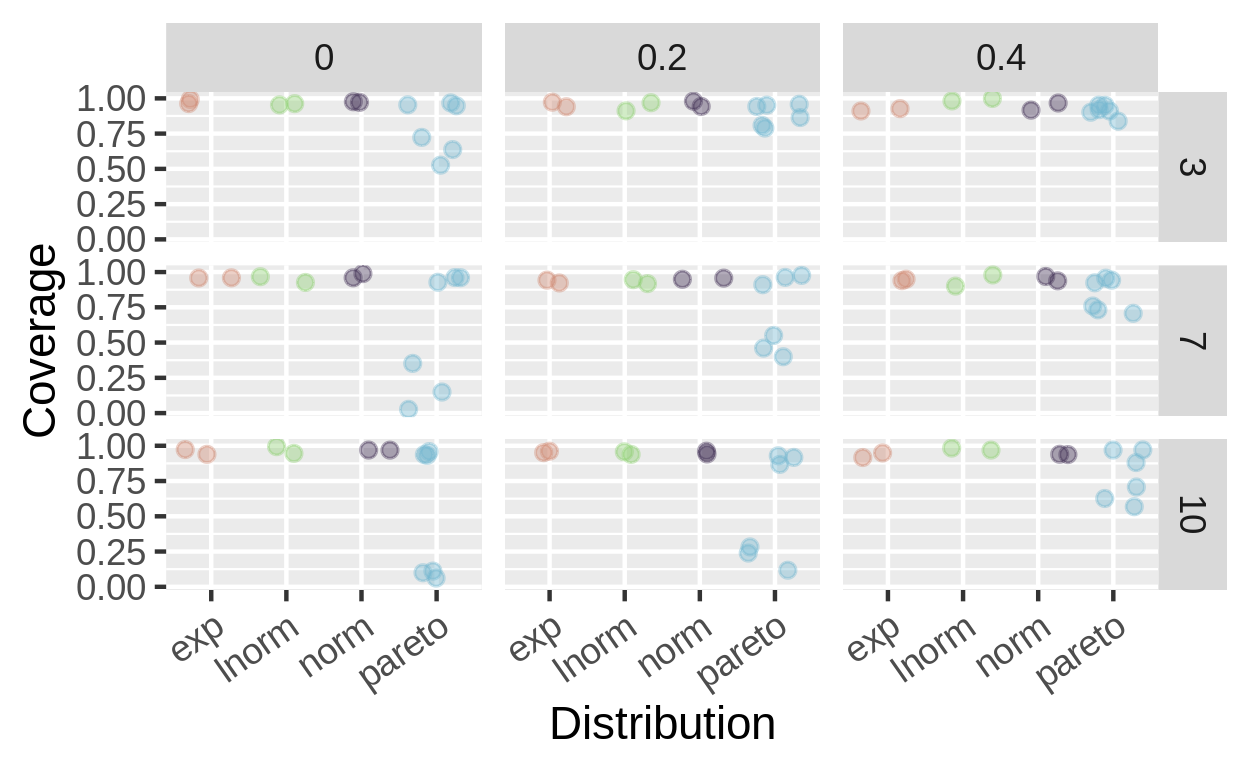
\includegraphics[width=1\linewidth]{eshplot} \end{center}

\vfill\null

This poster was created with
\texttt{posterdown::}\textcite{thorne_posterdown:_2019}.

\small\printbibliography
}
\end{adjmulticols*}
%------------------ Body End ---------------------%
%end the poster
\end{document}

